\chapter{Modelado y construcción del PCB.}
% ----------------------

\label{C:EModelado y construcción del PCB.}

\section{Software y herramientas de diseño empleadas.}

A partir de los circuitos desarrollados en los capítulos anteriores, se procedió a diseñar una placa de circuito impreso (PCB) personalizada. Esta placa está diseñada para integrar todos los componentes necesarios y crear un prototipo funcional que permita realizar ensayos sobre materiales en una superficie comprimida. \par 
La modelación y diseño del PCB se llevaron a cabo utilizando el software KiCad, reconocido por su amplia gama de herramientas de personalización de componentes. Este software permite a los diseñadores lograr un alto nivel de precisión y calidad en sus diseños, adecuándose a las habilidades específicas de cada usuario.\cite{kicad} \par 
El proceso de diseño incluyó la disposición estratégica de los componentes para optimizar el rendimiento del circuito, así como la consideración de factores como la disipación de calor, la integridad de la señal y la minimización de interferencias electromagnéticas. Además, se realizaron varias iteraciones del diseño para asegurar que el PCB final cumpliera con todos los requisitos técnicos y de funcionamiento necesarios para los ensayos planificados. \par 
El uso de KiCad facilitó la creación de un diseño detallado y eficiente, permitiendo visualizar en todo momento el aspecto final del PCB y realizar ajustes necesarios antes de proceder a su fabricación.

\section{Construcción del primer prototipo.}
La fase de construcción se inició con el desmontaje de la placa analógica de la fuente utilizada en un proyecto anterior que se puede apreciar en la Figura \ref{F:placa_original}, la cual se caracterizaba por sus atributos de control predominantemente analógicos. Este proceso permitió la recuperación de una variedad de materiales que, en su mayoría, se emplearían en el desarrollo del nuevo prototipo de fuente digital. Entre los componentes rescatados se encuentran resistencias, capacitores, disipadores de calor, borneras, entre otros. La reutilización de estos elementos fue posible gracias a la topología de la nueva fuente digital, que permitía su integración sin comprometer el diseño ni la funcionalidad del prototipo.  \par 
El proceso de desmontaje y reutilización de componentes se llevó a cabo meticulosamente, asegurando que cada pieza recuperada estuviera en condiciones óptimas para su reimplementación como se observa en la Figura \ref{F:desmontaje_de_la_placa}. Este esfuerzo contribuyó a la eficiencia del proyecto y a la racionalización de recursos, destacando la importancia de la sostenibilidad y la economía circular en el ámbito del diseño y construcción de dispositivos electrónicos.
\begin{figure}[H]
    \centering
    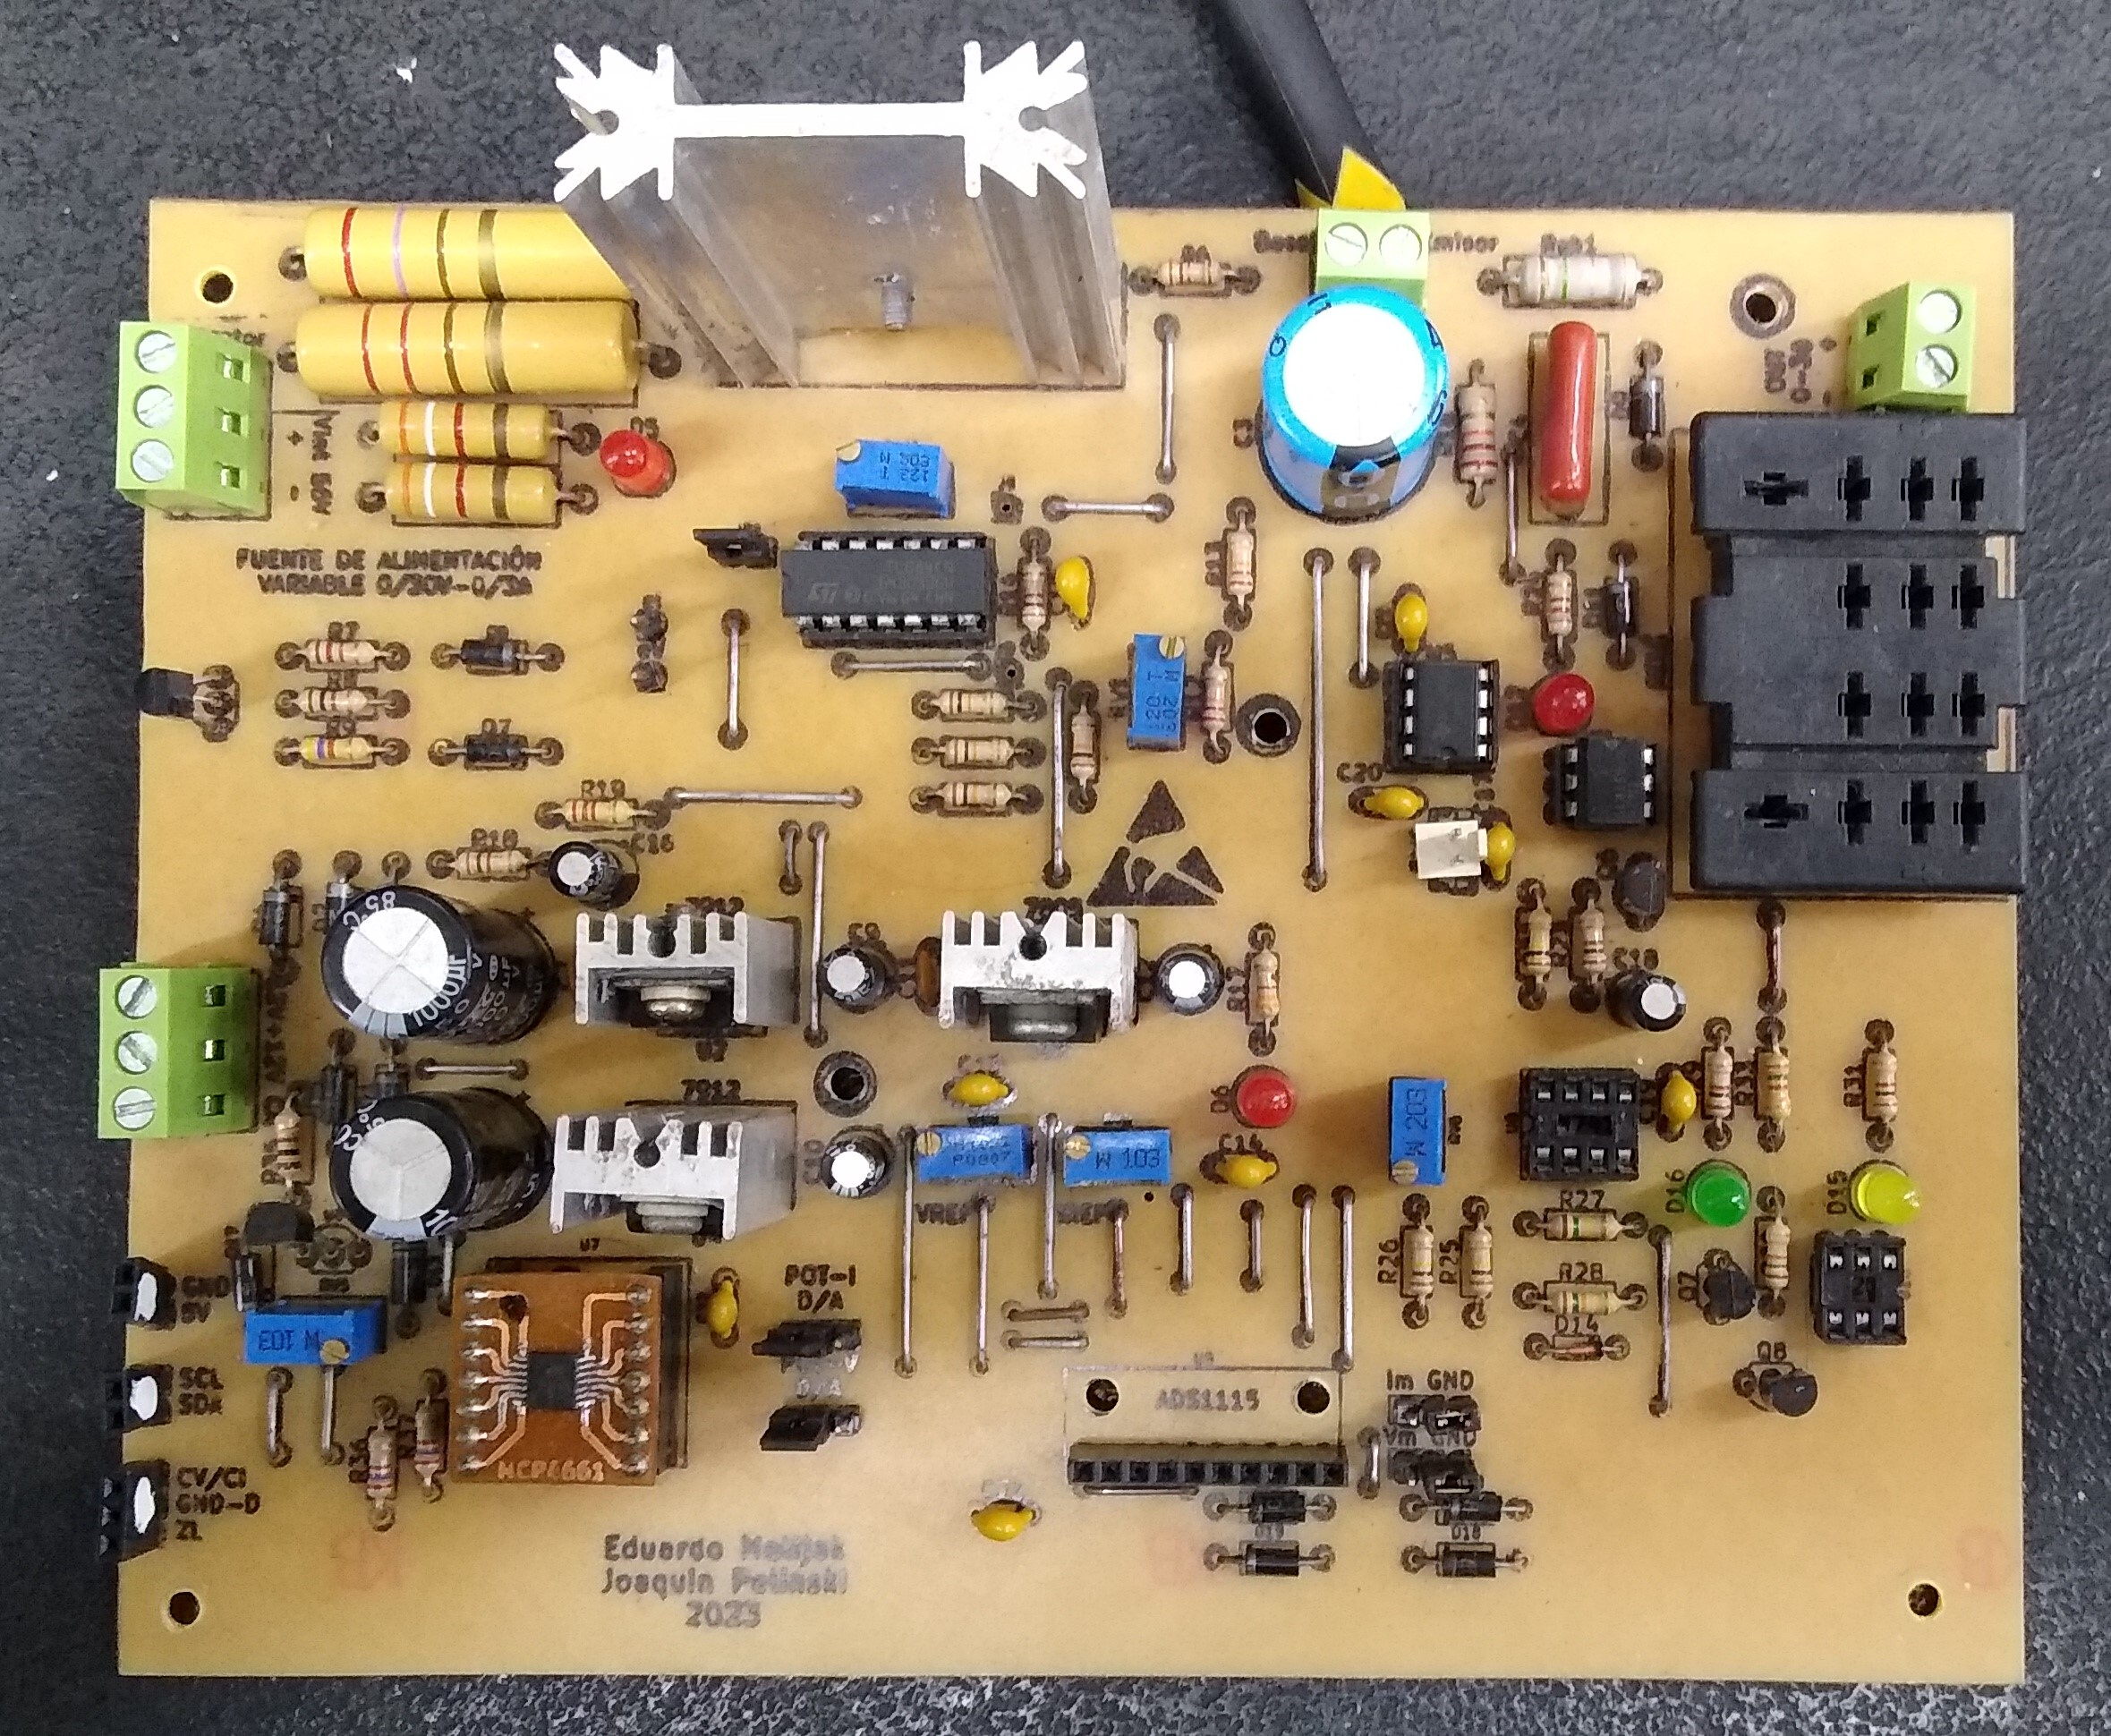
\includegraphics[width=0.8\textwidth]{./imagenes/fotos/placa_original.jpg}
    \caption{Antes del desmontaje de la placa de control analógica.}
    \label{F:placa_original}
\end{figure}

\begin{figure}[H]
    \centering
    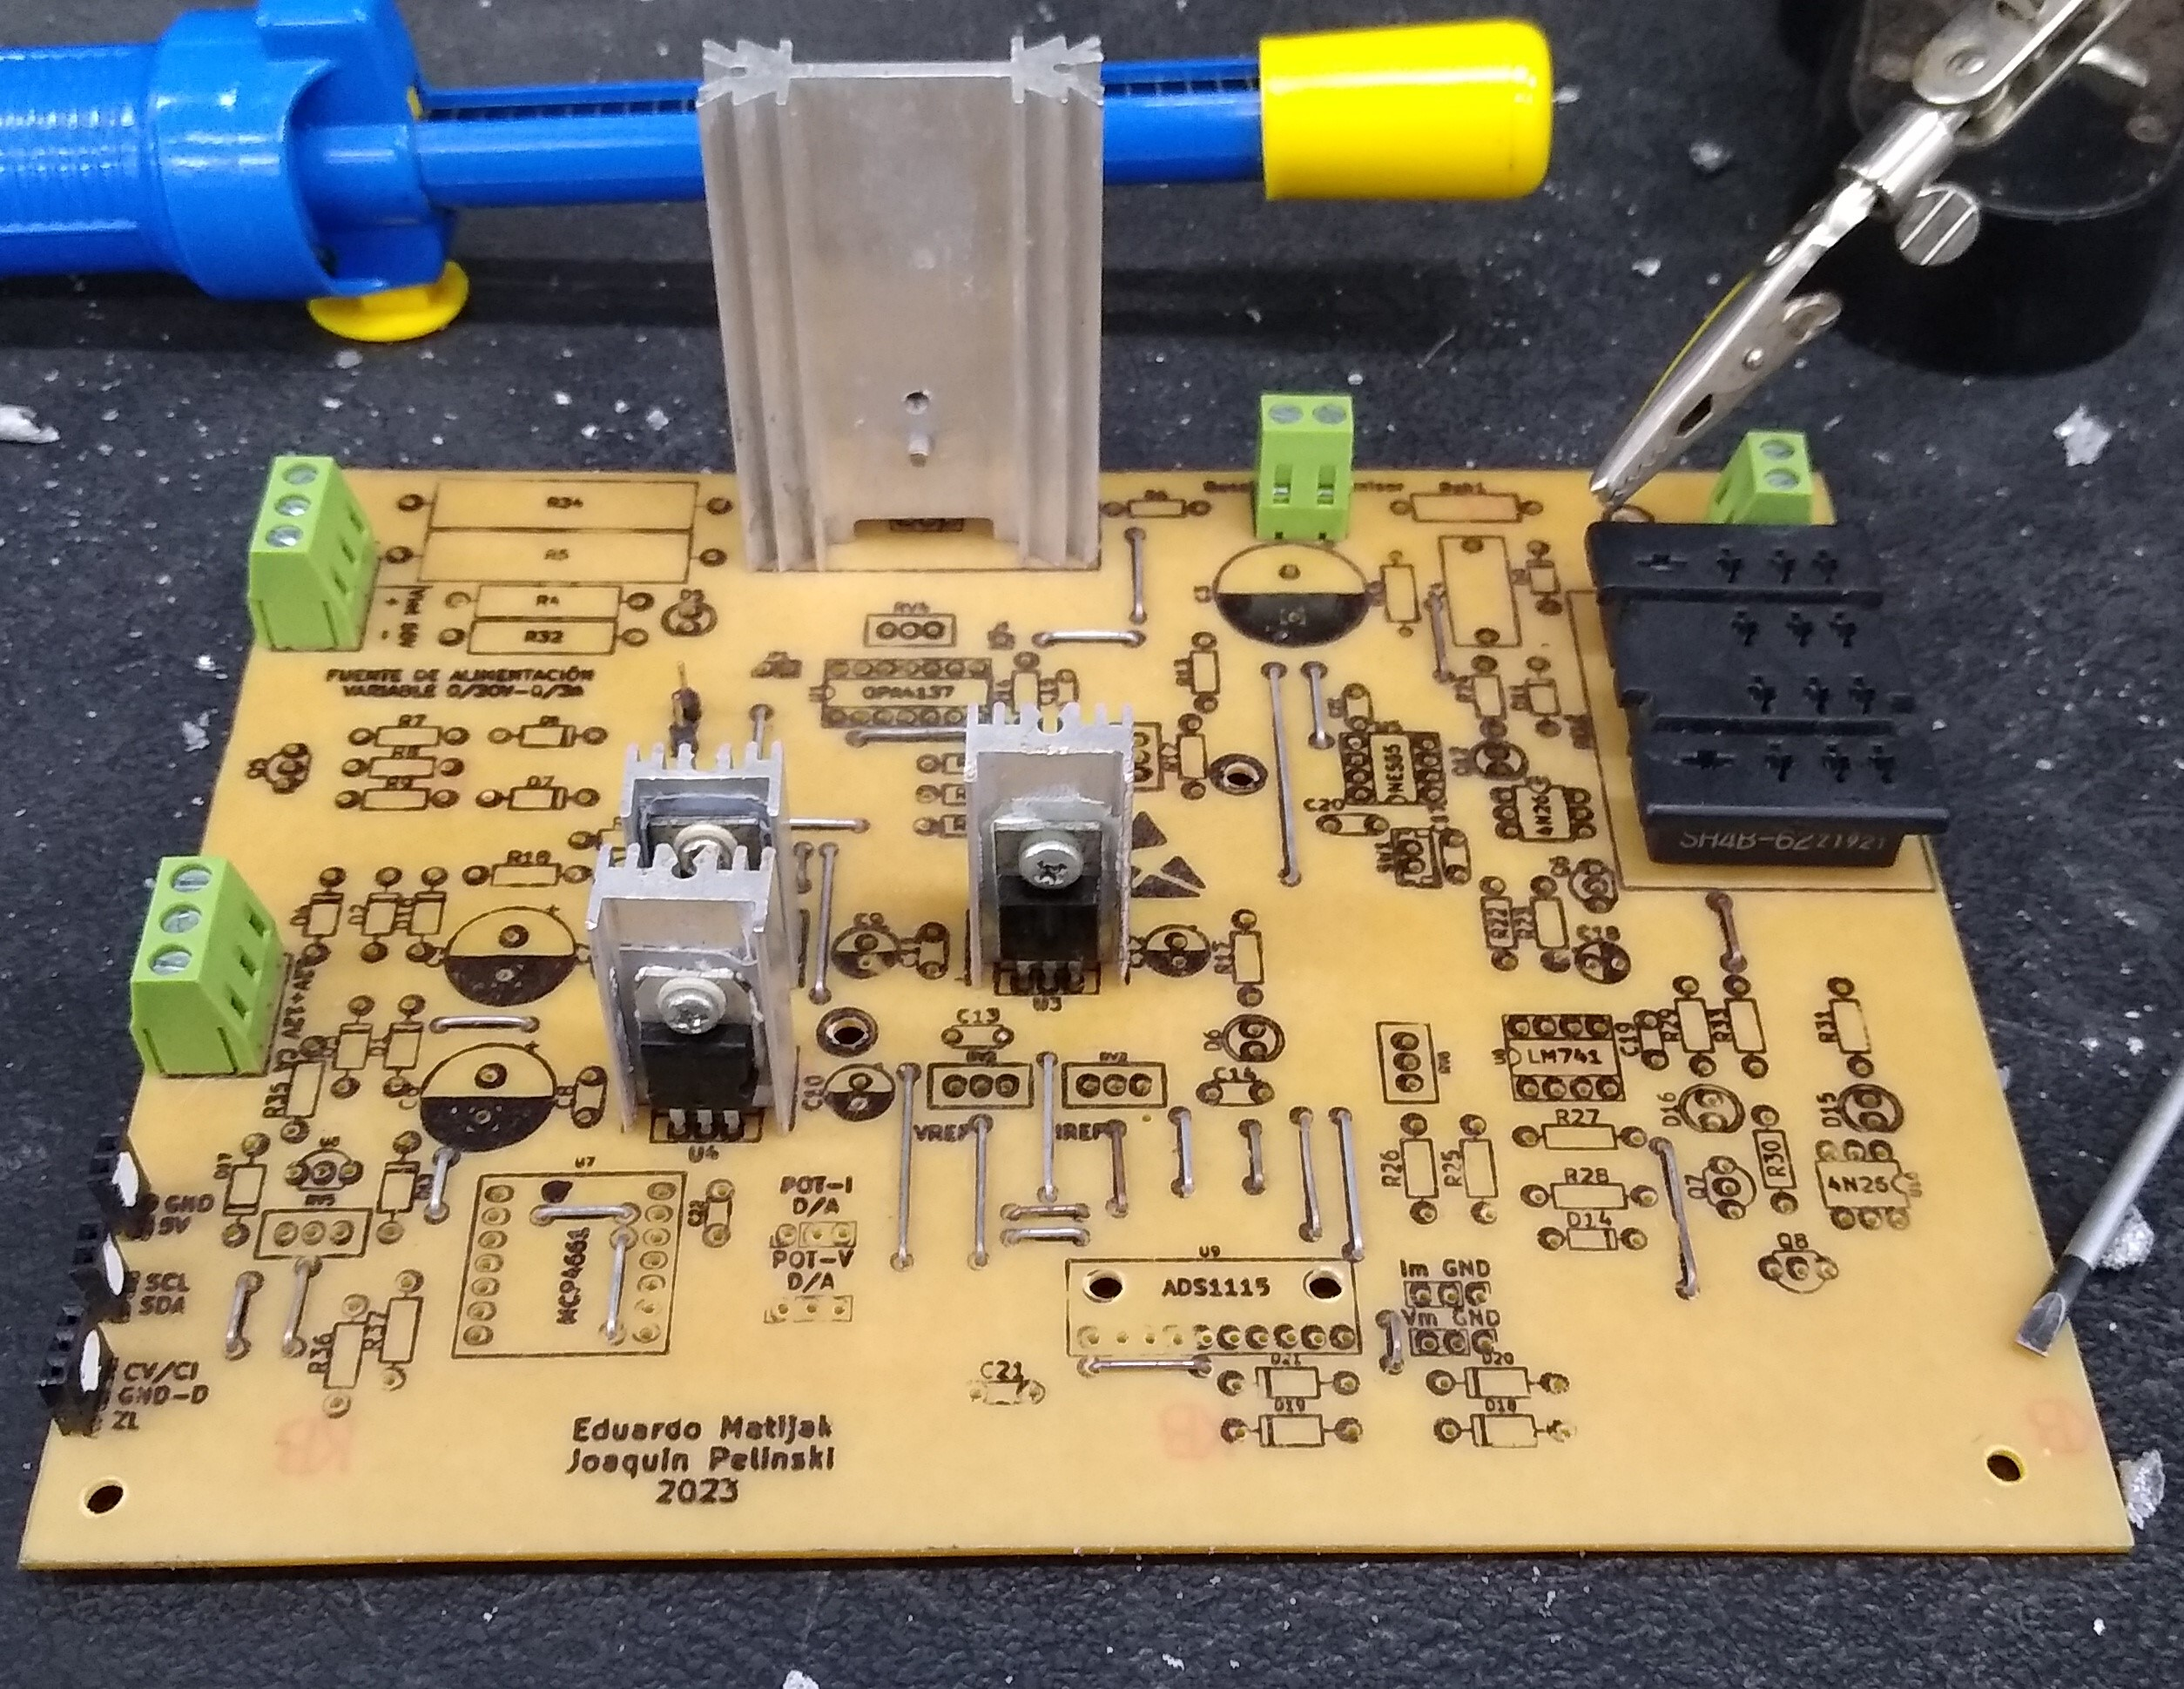
\includegraphics[width=0.8\textwidth]{./imagenes/fotos/desmontada.jpg}
    \caption{Después del desmontaje de la placa de control analógica.}
    \label{F:desmontaje_de_la_placa}
\end{figure}\par 
A continuación, se presenta el diseño del prototipo utilizado, el cual incorpora todos los elementos necesarios para la realización de las pruebas de funcionamiento. La característica principal de este PCB es su capacidad para integrar en un espacio compacto de 15x20 cm todos los componentes que anteriormente estaban dispersos en el modelo anterior. \par 
Una excepción notable en el diseño es la ubicación de la pantalla y el teclado, que se ha decidido mantener separados del PCB principal. Esta decisión se tomó debido a que no tendría sentido práctico incluir estos elementos directamente sobre la placa. En su lugar, se emplearon pines de salida, como borneras, para conectar estos componentes externos, facilitando su integración y operación. \par 
El diseño resultante, que se muestra en la Figura \ref{F:PCB_V1}, incluye también una representación tentativa en 3D del PCB. En esta representación se pueden observar las disposiciones de los componentes y la estructura general del prototipo. Es importante destacar que, para evitar daños y facilitar el acceso y reemplazo, algunos de los componentes están montados sobre tiras de pines hembra en lugar de estar soldados directamente sobre la placa. Esta configuración no solo mejora la durabilidad del prototipo, sino que también permite una mayor flexibilidad en la realización de pruebas y modificaciones. 
\begin{figure}[H]
    \centering
    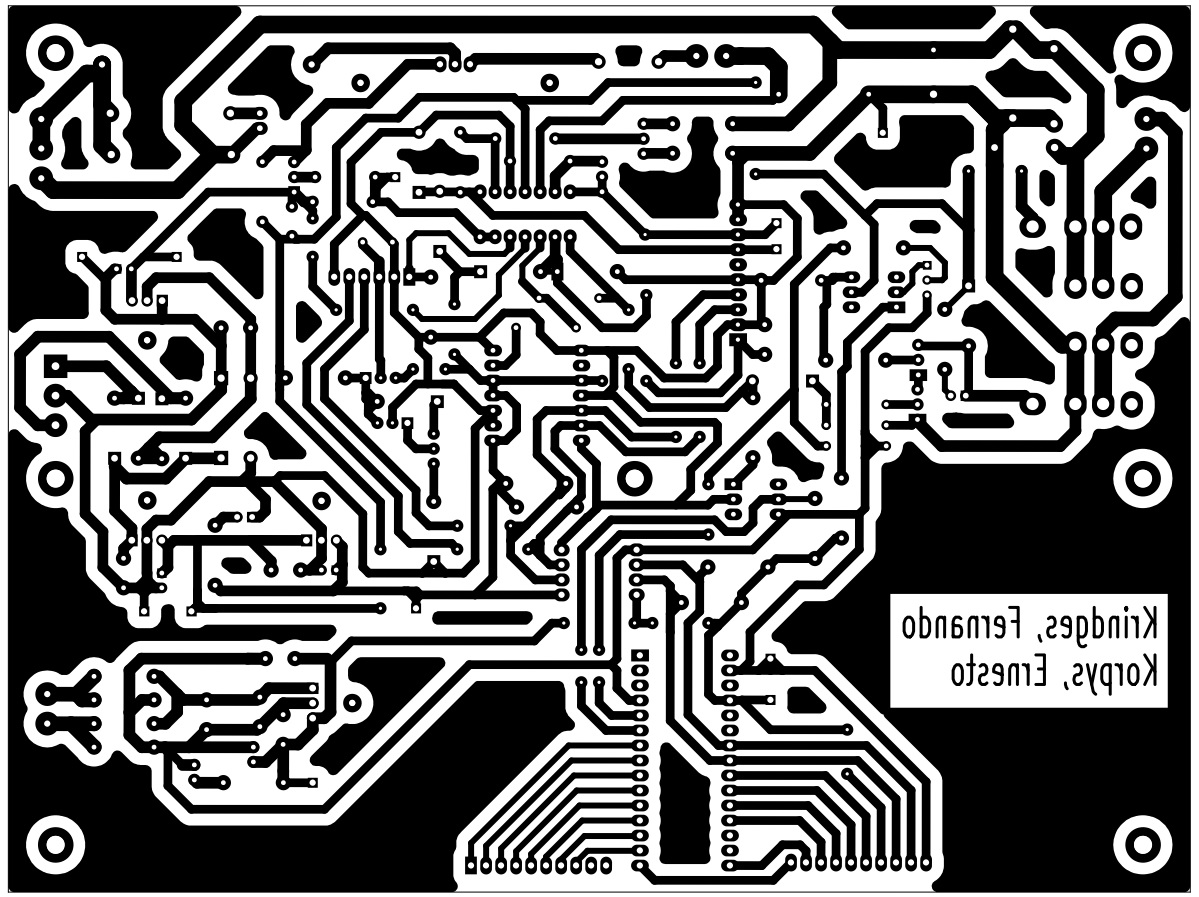
\includegraphics[width=\textwidth]{./imagenes/pcb_v1.jpg}
    \caption{Primer prototipo de PCB.}
    \label{F:PCB_V1}
\end{figure}
Se incluye un modelo 3D en el diseño con el fin de visualizar la disposición y la accesibilidad de los componentes, asegurando que el montaje y el mantenimiento del PCB sean lo más eficientes posible. Este es presentado en la Figura \ref{F:PCB_3D}.
\begin{figure}[H]
    \centering
    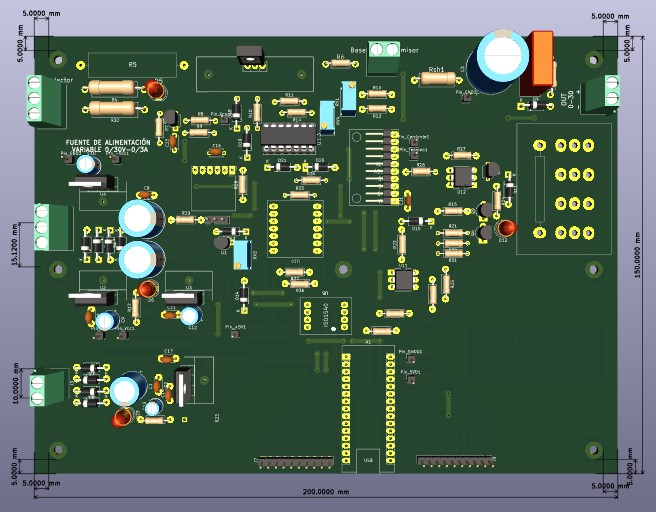
\includegraphics[width=\textwidth]{./imagenes/prototipo1.jpg}
    \caption{Vista 3D del primer prototipo.}
    \label{F:PCB_3D}
\end{figure} \par 
\begin{figure}[H]
    \centering
    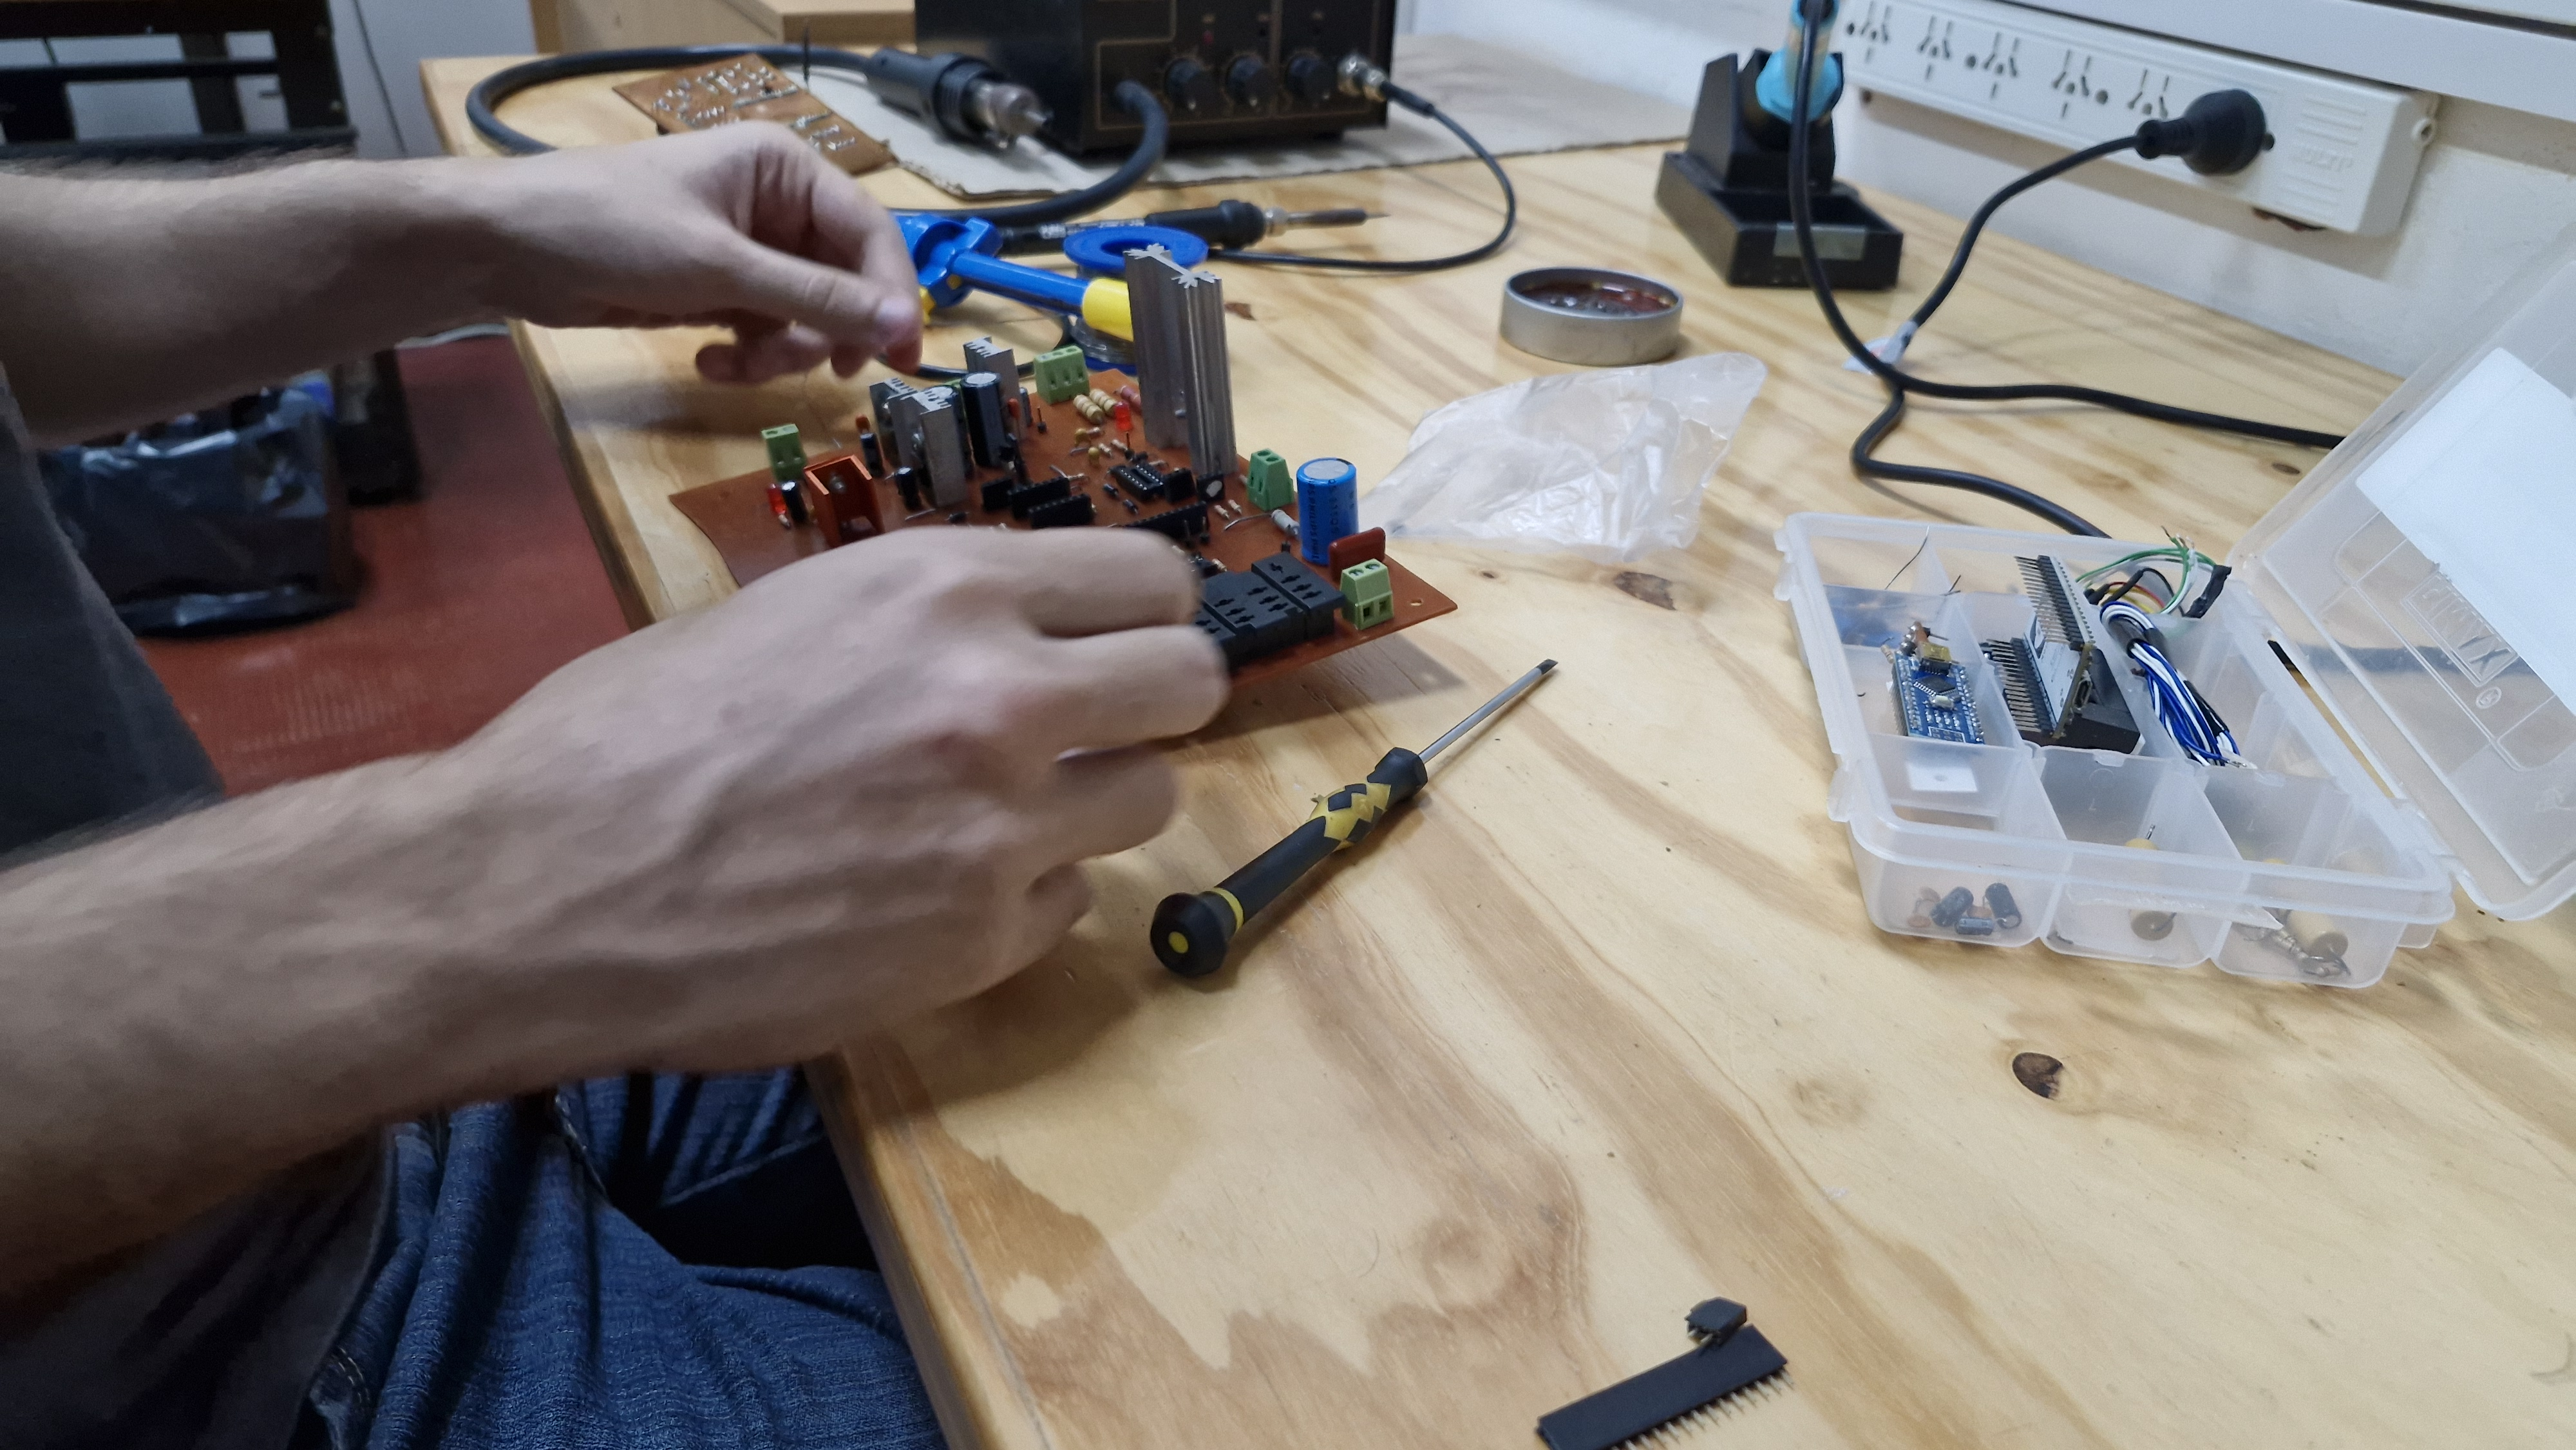
\includegraphics[width=\textwidth]{./imagenes/fotos/montaje.jpg}
    \caption{Montaje de los componentes en la placa.}
    \label{F:montaje_componentes}
\end{figure} \par 

\section{Ensayo de laboratorio y pruebas prácticas.}
Una vez verificada la continuidad de las pistas, el adecuado funcionamiento de los componentes, y los niveles de tensión en varios puntos clave, se procedió a energizar la fuente con todos los transformadores, tomando todas las precauciones necesarias para evitar daños a los componentes.\par 
A partir de este punto, se realizó una serie de pruebas y ajustes detallados para garantizar el correcto funcionamiento de la fuente. Estas pruebas incluyen la verificación de la respuesta del sistema bajo diversas condiciones de carga y la evaluación de la estabilidad del lazo de control. El uso del osciloscopio fue fundamental en este proceso, como se aprecia en la Figura \ref{F:esayos_y_pruebas}, ya que permitió observar en tiempo real cómo el lazo de control afectaba la salida de la fuente, aspecto crucial para el correcto desempeño del dispositivo.
Durante estas pruebas, se monitorizaron diversos parámetros, tales como la tensión de salida, la respuesta transitoria, y el comportamiento ante variaciones en la carga. Cada ajuste se realizó con el objetivo de optimizar la \textit{performance} del prototipo, asegurando que este cumpliera con los requisitos especificados y operara de manera eficiente y estable.\par 

\begin{figure}[H]
    \centering
    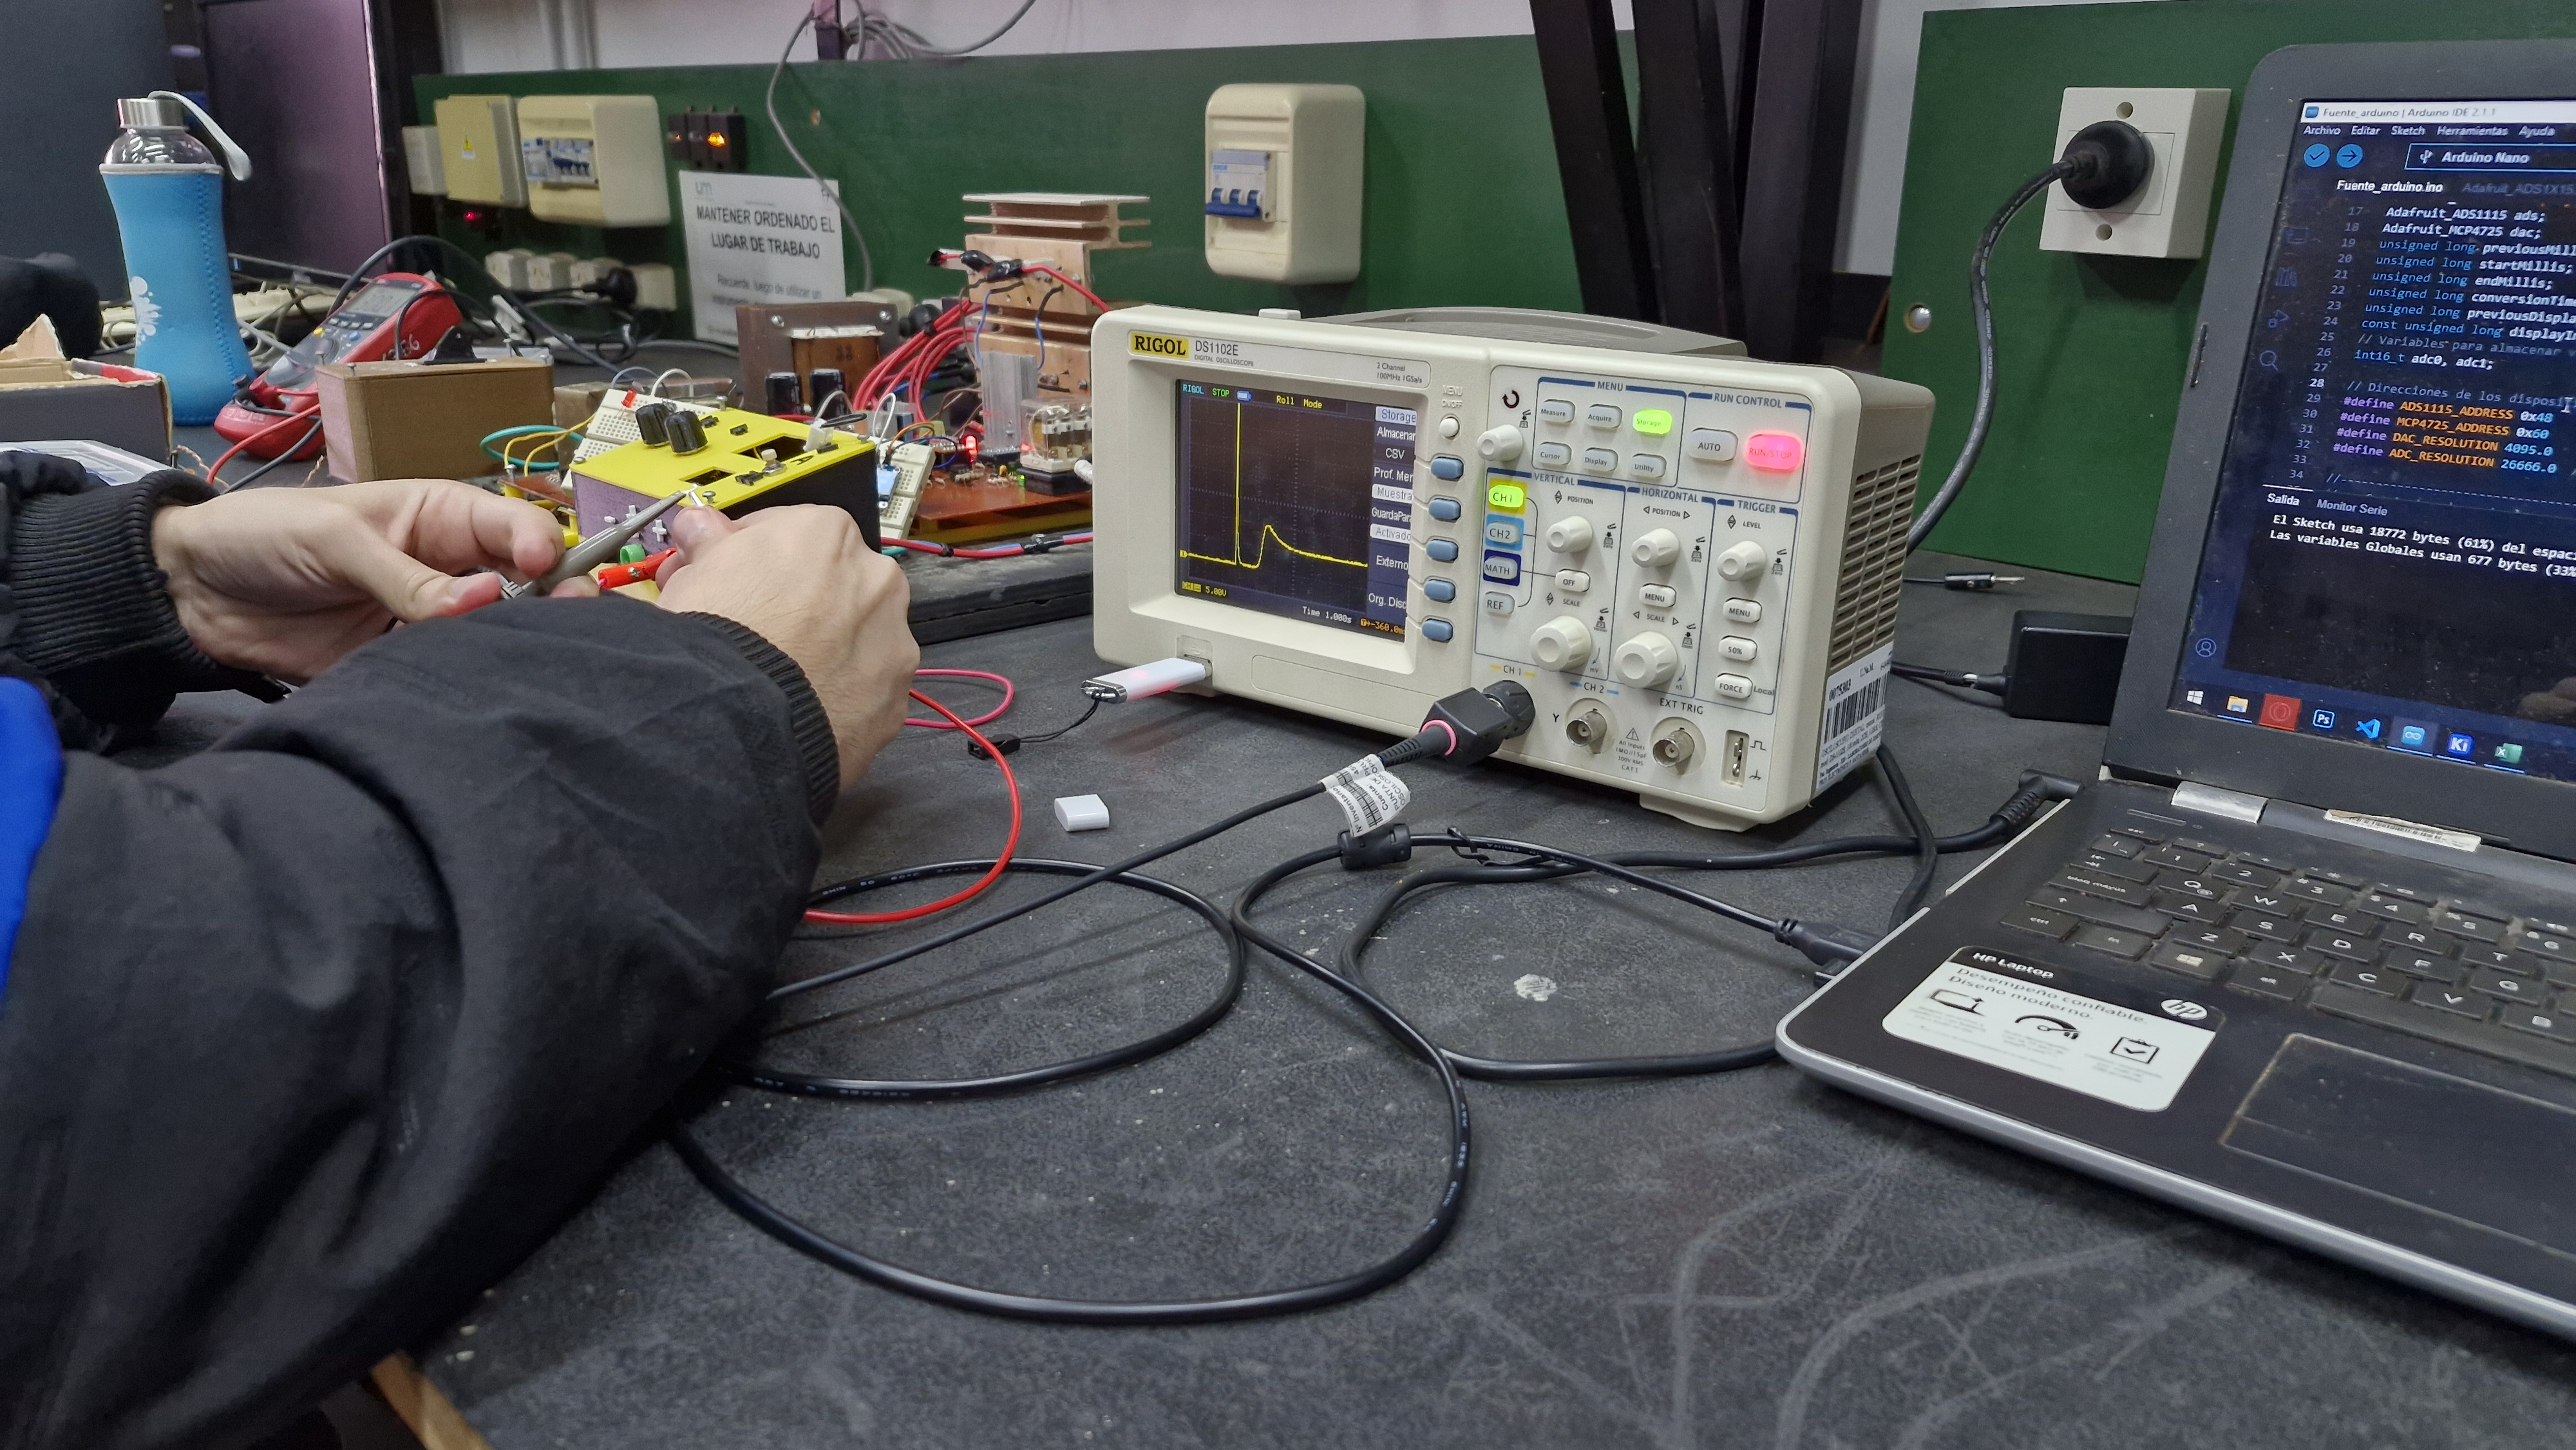
\includegraphics[width=0.9\textwidth]{./imagenes/fotos/osciloscopio.jpg}
    \caption{Ensayo con osciloscopio de la placa.}
    \label{F:esayos_y_pruebas}
\end{figure}
El resultado de estos ensayos fue satisfactorio, evidenciando que el diseño y la construcción del PCB fueron exitosos pero sin embargo no del todo concluyentes. Por lo que para la construcción del siguiente prototipo, se obtuvieron las siguientes observaciones que serán tomadas en cuenta.  \par 
\section*{Observaciones}
\begin{itemize}
    \item Los transistores comienzan a operar con una acción de control mínima de $0,3V$.
    \item Ante condición de vacío el capacitor de salida se carga y dispara su voltaje en cuestión de unos milisegundos, por lo que es necesario un control especial para contemplar este detalle.
    \item Cuando el DAC se inicializa establece su voltaje de salida en $2,5V$. Luego de analizar su hoja de datos, es posible escribir en su memoria EEPROM el valor por defecto con el cual iniciará.
    \item Hubo un error en la asignación de la huella del DAC, teniendo dos de sus pines invertidos entre sí.
\end{itemize}

\section*{Mejoras a realizar}
\begin{itemize}
    \item Ajuste de constantes de controlador.
    \item Ajuste de frecuencia de muestreo.
    \item Mejora de la estrategia de control.
    \item Arreglar la huella y el \textit{ruteo} de las pistas relacionadas al DAC.
\end{itemize}

